\section{资本资产定价模型}
\begin{enumerate}
    \item 请比较证券市场线和资本市场线。\\
    \sol\\
    资本市场线(CML)与证券市场线(SML),都描述了证券投资收益与风险之间的关系,横轴都是风险,纵轴都是收益,两条线都向右上方倾斜,表明高风险高收益。但仔细观察,发现它们在适用范围变量选择和应用作用等方面存在着区别。
    \begin{enumerate}[label=(\arabic*)]
        \item 适用范围不同。SML描述的是任何一种资产或者资产组合的期望收益与系统风险之间的关系,它是一个有效市场给出的定价,但实际证券的收益可能偏离SML;而CML则描述有效资产组合与总风险的关系,任何资产(组合)的期望收益不可能高于CML。
        \item 二者的风险变量选择不同。SML的横坐标是系统风险$\beta$,考虑的仅是总风险的一部分;而CML的横坐标是总风险$\sigma$,其中既包括系统风险又包括非系统风险。
        \item 二者在应用上有所不同。SML作为CAPM模型的图像形式,主要应用于资产定价,计算证券的期望收益;而CML主要用于确定市场组合,构造投资组合,因此CML也称为有效的资本配置线。
    \end{enumerate}
    \item 如果一种证券位于证券市场直线的上方,那它是被高估了还是低估了?\\
    \sol\\
    位于证券市场线上方,所以其期望收益应更高,但人们把它的价值定在证券市场线在该$\beta$值对应的期望收益上,所以是被低估了。
    \item 如果无风险收益率和市场预期收益率分别是6\%和11\%,某$\beta$值为1.1的证券预期收益率是多少?\\
    \sol\\
    由题知:$i = 6\%, E(R_m) = 11\%, \beta_j = 1.1$,则
    \[E(R_p) = i + [E(R_m) - i]\beta_j = 6\% + (11\% - 6\%) \times 1.1 = 11.5\%.\]
    故证券预期收益率是11.5\%。
    \item 设无风险利率为9\%,期望的市场回报率为15\%。试画出证券市场线,并指出进取型的证券位于何处,以及防御型的证券将位于何处?\\
    \sol\\
    由题知:$i = 9\%, E(R_m) = 15\%$,则
    \[E(R_p) = i + [E(R_m) - i]\beta_j = 0.09 + 0.06\beta_j,\]
    证券市场线方程为$E(R_p) = 0.09 + 0.06\beta_j$。\\
    证券市场线图如下:
    \begin{center}
        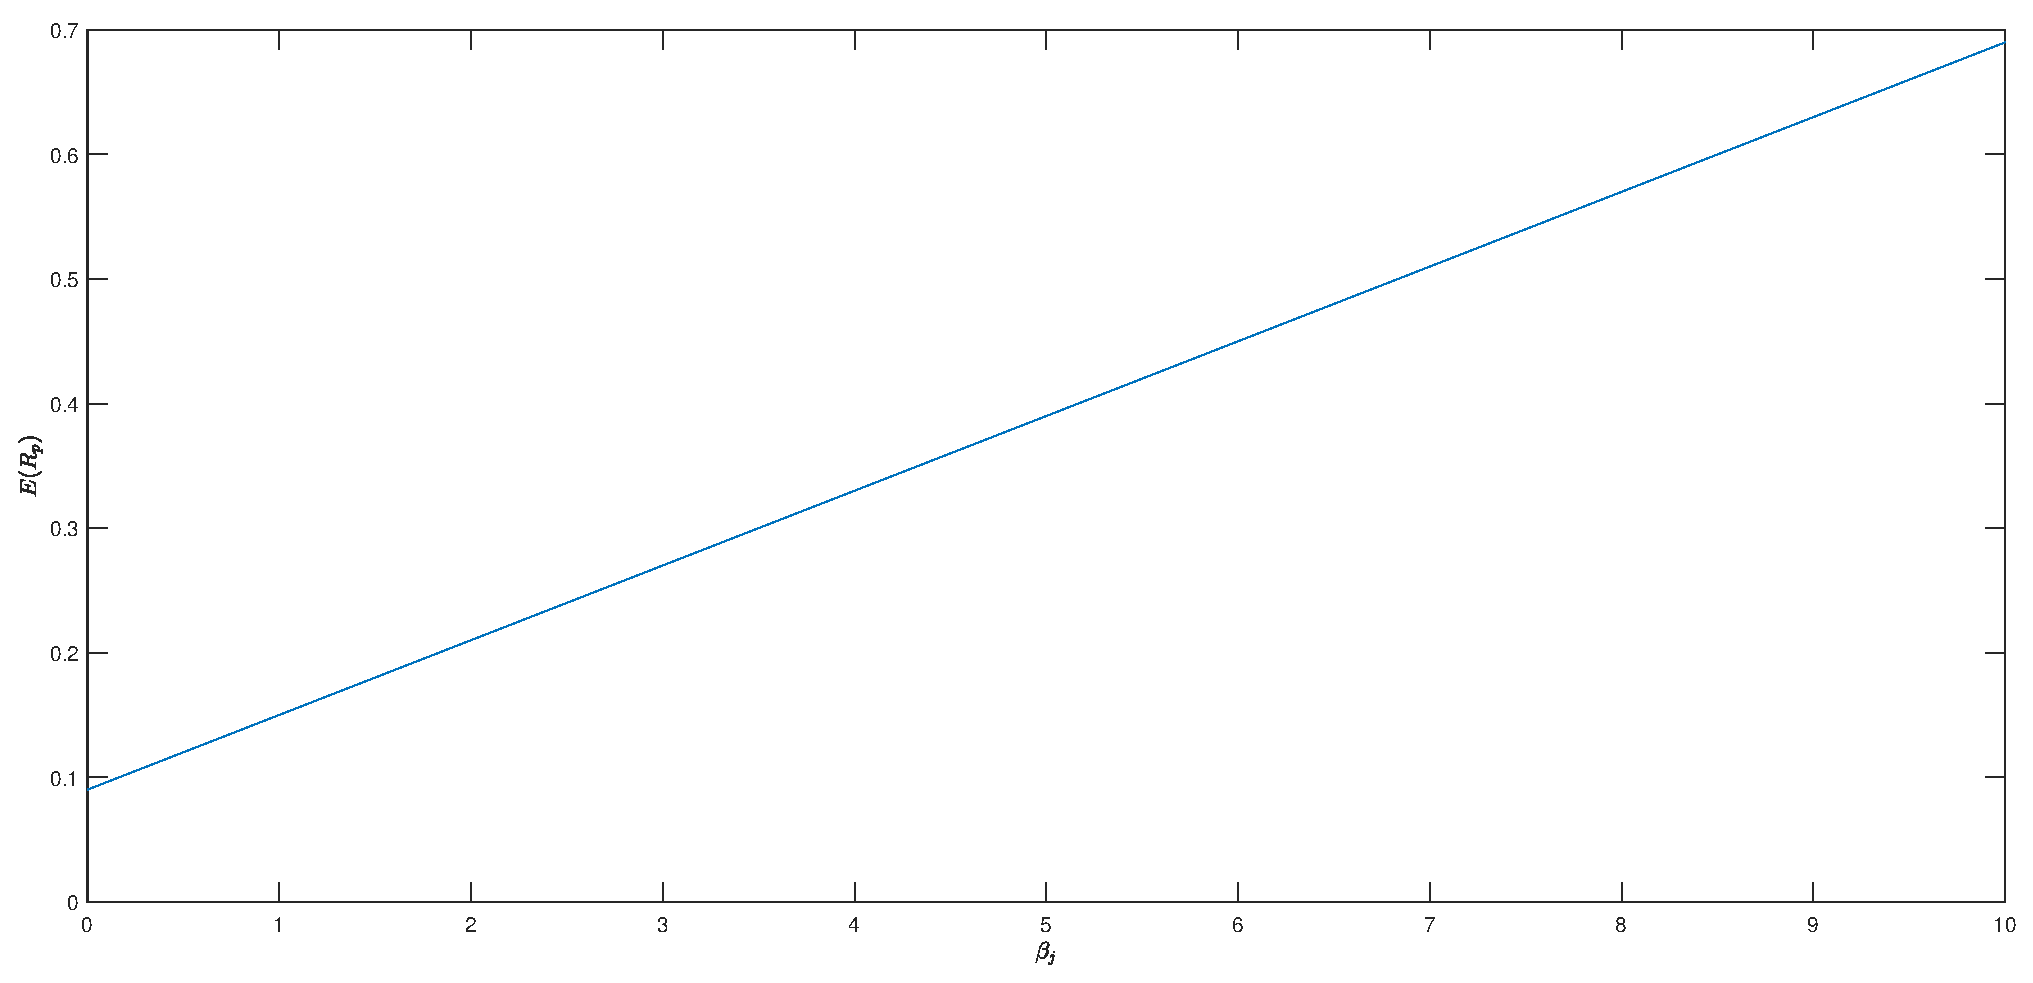
\includegraphics[scale=0.49]{3_4.eps}
    \end{center}
    进取型证券$\beta_j > 1$,其风险大于市场证券组合的风险,期望收益也大于市场证券组合的期望收益$E(R_m)$,其直线位于证券市场线的上方,被低估了;\\
    防御型证券$\beta_j < 1$,其风险小于市场证券组合的风险,期望收益也小于市场证券组合的期望收益$E(R_m)$,其直线位于证券市场线的下方,被高估了。\\
    Matlab绘图命令如下:
\begin{lstlisting}
x = 0:0.001:10;
y = 0.09 + 0.06 * x;
plot(x, y);
\end{lstlisting}
% xlabel('$\beta_j$', 'interpreter', 'latex');
% ylabel('$E(R_p)$', 'interpreter', 'latex');
    \item 证券$L$的$\beta$值为0.70,而证券$K$的$\beta$值为1.30。运用上题的有关证券市场直线的数据,计算各证券的期望回报率。\\
    \sol\\
    由上题:$i = 9\%, E(R_m) = 15\%$,则证券$L$的期望回报率为
    \[E(R_L) = 0.09 + 0.06 \times 0.7 = 13.2\%,\]
    故证券$L$的期望回报率为13.2\%。\\
    证券$K$的期望回报率为
    \[E(R_K) = 0.09 + 0.06 \times 1.3 = 16.8\%,\]
    故证券$K$的期望回报率为16.8\%。
    \item 证券$A$、$B$的预期收益率和$\beta$值见下表:
    \begin{center}
        \setlength{\tabcolsep}{21mm}{
        \begin{tabular}{c|c|c}
            \hline
            证券 & 预期收益率/\% & $\beta$值 \\ \hline
            $A$ & 14.80 & 16.30 \\ \hline
            $B$ & 1.24 & 1.82 \\ \hline
        \end{tabular}}
    \end{center}
    如果市场收益率是12.5\%,无风险收益率是3.6\%,哪一只证券更值得购买?\\
    \sol\\
    由CAPM模型,$A$、$B$两证券在市场均衡时的期望收益率为
    \begin{align*}
        & E(R_A) = 3.6\% + (12.5\% - 3.6\%) \times 16.3 = 148.67\% > 14.80 \%, \\
        & E(R_B) = 3.6\% + (12.5\% - 3.6\%) \times 1.82 = 19.798\% > 1.24 \%.
    \end{align*}
    显然,$A$、$B$证券实际投资的期望收益率均低于市场均衡时的期望收益率,且$B$证券两者的期望收益率之差更接近0,则$B$证券更值得购买。
    \item 用实证分析检验CAPM模型。\\
    \omitted
    \item 假设市场证券组合的期望收益为9\%,标准差为30\%,市场利率为3\%,求证券市场线的方程,假设证券$A$的$\beta$值为0.6,根据CAPM模型计算该证券的期望收益。若证券$B$的标准差为0.6,其与市场证券组合的相关系数为0.25,根据CAPM模型,计算该证券的期望收益率。\\
    \sol\\
    由题知:$i = 3\%, E(R_m) = 6\%$,则
    \[E(R_p) = i + [E(R_m) - i]\beta_j = 0.03 + 0.03\beta_j,\]
    故证券市场线方程为$E(R_p) = 0.03 + 0.03\beta_j$。\\
    证券$A$的$\beta_A = 0.6$,则
    \[E(R_A) = 0.03 + 0.03 \times 0.6 = 4.8\%,\]
    故证券$A$的期望收益为4.8\%。\\
    证券$B$的$\displaystyle\beta_B = \frac{\rho_{Bm}\sigma_B}{\sigma_m}=\frac{0.25 \times 0.6}{0.3}=0.5$,则
    \[E(R_B) = 0.03 + 0.03 \times 0.5 = 4.5\%,\]
    故证券$B$的期望收益为4.5\%。
    \item 假设股票$A$的风险为0.32,$\beta$值为1.42,而股票$B$的风险为0.68,$\beta$值为0.75。哪个股票的总风险更大呢?哪个股票的市场风险更大?假设市场利率为2\%,市场期望收益率为10\%,哪个公司\textcolor{red}{(公司改为股票)}的价值更高?\\
    \sol\\
    由题知:$\sigma_A^2 = 0.32, \beta_A = 1.42, \sigma_B^2 = 0.68, \beta_B = 0.75$,则
    \begin{align*}
        & \sigma^2(R_A) = \beta_A^2 \sigma_A^2 = 0.32 \times 1.42^2 = 0.645248,\\
        & \sigma^2(R_B) = \beta_B^2 \sigma_B^2 = 0.68 \times 0.75^2 = 0.3825.
    \end{align*}
    故股票$A$的总风险、市场风险更大。
    \begin{align*}
        & E(R_A) = 0.02 + (0.1 - 0.02) \times 1.42 = 0.1336,\\
        & E(R_B) = 0.02 + (0.1 - 0.02) \times 0.75 = 0.08.
    \end{align*}
    故股票$A$的价值更高。
\end{enumerate}
\clearpage